\chapter{Detailed Design}
\label{chp:DetailedDesign}
This chapter documents the detailed design of the Ear-Monitor's subsystems. The hardware and software sides are discussed separately. 

\section{Hardware}

A typical telemedicine configuration is used for the Ear-Monitor and its supporting system. It is similar to the configuration used by \cite{wang2010wearable} and \cite{prawiro2016integrated} for their respective wearable health monitors. The ear-probe is the signal acquisition module of the Ear-Monitor and contains the sensors. A microcontroller unit (MCU) is used to control the flow of data within the Ear-Monitor and data is sent by means of a wireless transceiver to a device running supporting software, where data is stored for later access. Figure \ref{fig:HardwareFlowchart} illustrates the flow of information through the hardware set-up.

\begin{figure}[h]
\centering
\graphicspath{{figs/}}
\input{figs/HardwareFlowchart.pdf_tex}
\caption{Flow of information in a typical telemedicine set-up}
\label{fig:HardwareFlowchart}
\end{figure}

This section documents the detailed design of each of the key parts of hardware found in the Ear-Monitor.

\subsection{Temperature sensor}
The non-contact, IR TMP006 is selected to measure tympanic membrane temperature in the Ear-Monitor. Four wires are connected for power and serial communication lines. The package has eight solder balls for surface mounting on a printed circuit board (PCB). A big challenge was to mount this micro-component. Various methods were tested:

\begin{itemize}
\item A PCB was designed and manufactured, but mounting the miniature TMP006 on this PCB proved to be problematic.
\item The device footprint and wire connection pads were etched into copper clad flexible circuit board sheets. Solder paste and a heat gun was used to mount the TMP006. This method worked, but mounting proved to be unreliable, for connections were sometimes not made properly or the TMP006 got damaged.
\item Pre-mounted boards were acquired and the excess material were cut away to allow wires to be soldered to the exposed tracks.
\end{itemize}

\medskip

This last method proved to be the best solution for the proof of concept version of the Ear-Monitor. It was necessitated by the lack of advanced facilities to mount micro SMT components. The flexible circuit board method will be preferable when a SMT component placement system is available. Figure \ref{fig:TMP006_Breakout} shows the bought, pre-mounted boards and the cut-out component along with the four connections. 3.3V and ground (GND) are connected to a power regulator and the two serial communication wires are connected to the serial communication I/O pins of the MCU.

\begin{figure}[h]
\centering
\graphicspath{{figs/}}
\input{figs/TMP006_Breakout.pdf_tex}
\caption{(a) TMP006 pre-mounted boards and (b) the cut-out sensor segment with four connections labeled}
\label{fig:TMP006_Breakout}
\end{figure}

According to the TMP006's user guide, the sensor captures radiation form almost its entire 180\textdegree{} field of view (FOV), but the majority of the received signal comes from sources that are parallel to, and precisely in front of the sensor. The final target object temperature is an integration of all the radiation signals captured across the FOV of the sensor.

\medskip

The user guide also states that the smaller the object is, the closer it should be placed to the sensor to prevent other objects from entering the field of vision. The goal is to place the sensor at least 5mm from the membrane. This will remove the risk of contact with the membrane, while still ensuring thermal radiation from the canal is detected. Energy from the ear canal self will inevitably be detected by the sensor, but the majority of the radiation will come from the membrane and it is assumed that the wall near the membrane is in thermal equilibrium with the membrane within an acceptable margin. To achieve this position, the TMP006 will be placed at the tip of the ear probe.

\medskip

Energy radiated or conducted between the PCB and the sensor can cause temperature calculation errors. To prevent this the sensor and PCB should be kept at the same temperature. The ear probe set-up of the Ear-Monitor is favourable for this task, for the PCB is very small and contains no other heat generating components. Also, the target object, tympanum, will stay at a constant temperature, so the sensor will experience no heat fluctuations. It will, however, be necessary to allow time for the sensor and PCB to reach thermal equilibrium once placed inside the ear canal, before accurate measurements can be taken. This will not be a problem, for the device is designed to be worn continuously for long periods of time.

\subsection{Pulse Oximeter}
The MAX30100 pulse oximeter is selected to record red and IR photoplethysmographs from inside the ear canal. These are used for determining heart rate and SpO\textsubscript{2}. The MAX30100 is controlled with 5 connection wires, connected to 7 of the package's 14 pins. Figure \ref{fig:MAX30100_pinout} shows a diagram of the MAX30100 package and the required connections for operation. 3.3 V, 1.8 V an GND are connected to a power regulator and the two serial communication lines are connected to the serial communication I/O pins of the MCU.

\begin{figure}[H]
\centering
\graphicspath{{figs/}}
\def\svgwidth{180pt}
\input{figs/MAX30100_pinout.pdf_tex}
\caption{MAX30100 package diagram with required connections for operation.}
\label{fig:MAX30100_pinout}
\end{figure}

As with the TMP006, the mounting of the extremely small MAX30100 was a great challenge. The first attempt was to design and manufacture a PCB on the typically used, 1.6 mm thick, FR4 PCB material. This PCB proved to be too thick and its inflexibility caused extra problems in ensuring firm contact with the ear canal wall. The solution was to etch the footprint, tracks and pads into flexible circuit board material. The etching process involves:
\begin{itemize}
\item Design the layout on EAGLE PCB open source software.
\item Print the mirrored layout on toner transfer paper.
\item Preparing the copper clad material by cleaning with rubbing alcohol.
\item Transfer the ink form the toner transfer paper to the copper clad material by applying heat and pressure.
\item Submerge the copper clad material with ink layout in ferric chloride (FeCL\textsubscript{3})
\item Cleaning off the remaining ink with acetone to reveal the copper tracks.
\end{itemize} 

The ferric chloride dissolves all the copper that is exposed, leaving copper tracks that were covered by the ink during etching. The flexible copper clad material is \SI{60}{\micro\meter} thick, making it ideal for the size limitations inside the ear canal. Figure \ref{fig:MAX30100_layout} shows the layout designed and resulting etched flexible circuit board. The flexible nature of the circuit board allows it to be folded in halve to form a two sided circuit board, saving space and placing the all connection pads on the same end. It also allows for uniform and firm contact between the MAX30100 and the ear canal wall. Wires for power and communication are soldered to the five connection pads.

\begin{figure}[H]
\centering
\graphicspath{{figs/}}
\def\svgwidth{180pt}
\input{figs/MAX30100_layout.pdf_tex}
\caption{(a) is the layout as designed on EAGLE PCB  with the outline of the MAX30100 shown in black and (b) is the finished flexible PCB with copper tracks (insert scale?)}
\label{fig:MAX30100_layout}
\end{figure}

\subsection{Control and Communication Hardware}
The remaining electronic components consisted of the Arduino MCU, HC-05 Bluetooth modem and battery. A PCB is designed to integrate all the the different hardware subsystems. Additional electronics include the power regulators, I\textsuperscript{2}C pull-up resistors and a charging circuit for the LiPo battery. A on-off switch and power-on indicator LED are also added. 

\medskip

\SI{10}{\kilo\ohm} pull-up resistors on the SDA and SCL lines are recommended for standard I\textsuperscript{2}C communication and are therefore included in the design. A \SI{7.4}{\volt}, \SI{1000}{\milli\ampere\hour} rechargeable LiPo battery (https://www.robotics.org.za/603450?search=battery) is selected to supply power to the Ear-Monitor. The Ear-Monitor will be operate for XXX minutes on a sigle charge (Calculations in Appendix Y). The Arduino has its own power regulation circuitry on board and can be connected directly to the battery. Two low drop-out voltage regulators are selected to supply 1.8 V and 3.3 V to the sensors and Bluetooth modem. A charging circuit is added to allow the battery to be charge without physically disconnecting it from the device. Decoupling capacitors are added to all power supply lines. Figure \ref{fig:Ear-Monitor_BlockDiagram} shows block diagram of the Ear-Monitor's hardware. The diagram is split between the components on the PCB worn on the hear and the components in the ear probe.

\begin{figure}[H]
   \centering
   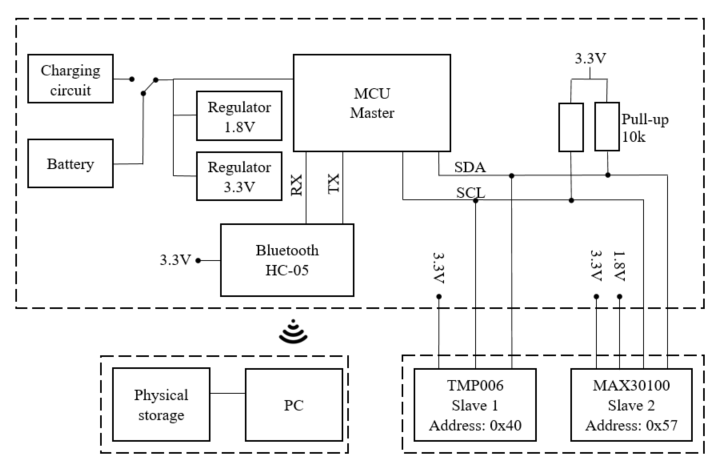
\includegraphics[scale=0.9]{figs/Ear-Monitor_BlockDiagram.png}
   \caption{Block digram for the Ear-Monitor's hardware components}
   \label{fig:Ear-Monitor_BlockDiagram}
\end{figure}

A schematic diagram and PCB layout is included in Appenxix (X). Calculations to select passive components is included in Appendix Y. The MCU, battery, Bluetooth modem and PCB will be worn in a headband around the head in this proof of concept version of the Ear-Monitor. Only the TMP006 and MAX30100 will be located at their correct positions in the ear canal hold in place by the ear probe. The ear probe is connected by a wire to the electronics in the headband. Data is sent from the headband to the PC through the wireless connection. It is well within the abilities of the current state of technology to reduces the size of all the electronics to a hearing aid, or even ear probe size device. But such miniaturisation is not within the scope of this project.

\medskip

An ear probe is designed to hold the MAX30100 and TMP006 in the correct positions in the ear canal and restrict their movement to minimize artefacts. Sugru\textsuperscript{\textregistered} is the band name for a mouldable silicone elastomer which is perfect for this application. According to the product documentation it is non-toxic and does not cause skin irritation. The mouldable putty is pressed into the ear and assumes the its shape, but does not conform completely, therefore allowing it to fit in different ear shapes. When cured, it has a sturdy, but flexible structure. Slots and holes are cut into the moulded probe to hold the sensors and wires. Figure \ref{fig:EarProbe} shows a photo of the completed ear probe.

\begin{figure}[H]
   \centering
   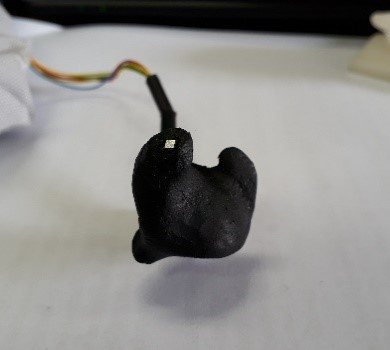
\includegraphics[scale=1]{figs/EarProbe.jpg}
   \caption{}
   \label{fig:EarProbe}
\end{figure}

Add a photo of the completed electronic hardware




\section{Software}
Software is written for the MCU and for the PC receiving and storing the data. MCU software is C++ based and developed using the Arduino IDE. MCU software handles sensor communication, timing, some processing and transmitting collected data via the Bluetooth modem. The PC software is Java based and developed using the Processing IDE. The PC software listens on the Bluetooth serial port, processes received data, display the data via a user interface and stores the received data on the local hard drive.

\medskip

Figure \ref{fig:Software_BlockDiagram} shows a diagram of the flow of data through the various software functions. The final calculated medical signs are shown in blue. The diagram is split between the MCU functions and PC functions. MCU and PC software are connected through the Bluetooth connection. The main functions are discussed in this section.

\begin{figure}[H]
   \centering
   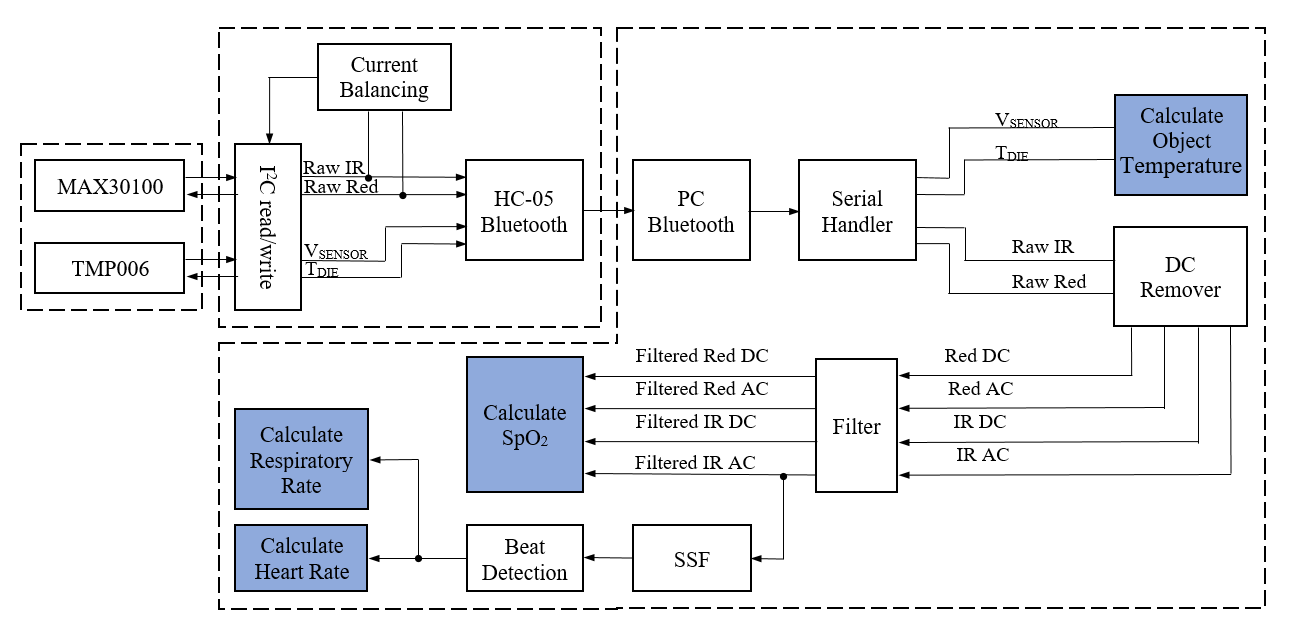
\includegraphics[scale=0.45]{figs/Software_BlockDiagram.png}
   \caption{Block diagram showing the flow of information through the various software functions. Final calculated medical signs are shown in 	blue}
   \label{fig:Software_BlockDiagram}
\end{figure}

\subsection{Sensor Communication Software}
Software is written for the MCU to communicate with the sensors and Bluetooth module. The MAX30100 and TMP006 have different default addresses and can share one I\textsuperscript{2}C bus for communication with the MCU. I\textsuperscript{2}C communication happens one byte at a time with no parity and MSB first. The eighth bit of the address indicates a read or write request. Figure \ref{fig:I2C_Read} shows how the software reads 16-bit values from the TMP006 registers. Values form the MAX30100 are read in a similar way.

\begin{figure}[H]
   \centering
   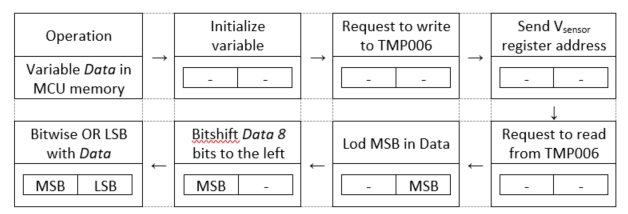
\includegraphics[scale=1]{figs/I2C_Read.png}
   \caption{How the software reads 16-bit values from the TMP006 registers}
   \label{fig:I2C_Read}
\end{figure}

Communication with sensors consists of two steps, configuration and reading data.

\subsubsection{Sensor Configuration}
Upon power on, both sensors start with default configurations. The MCU is programmed to reconfigure both sensors on start-up. This is done by writing values to the various configuration registers.
The MAX30100 is set to SpO\textsubscript{2} mode with \SI{1600}{\micro\second} LED pulse width, 50 Hz sampling rate and \SI{50}{\milli\ampere} current supply to both LEDs. The TMP006 is set to use the average of 16 conversions per output, meaning it will sample at 0.25 Hz. This is done, because the application does not demand a high sampling rate and increasing the number of samples per output will reducing noise (\SI{0.125}{\celsius}). These configurations are done every time the Ear-Monitor is powered on.

\subsubsection{Reading data from sensors}
After configuration is done, the MCU enters a continuous loop of sensor data reading. The MAX30100 uses one FIFO register to store the latest 16 IR and red photo-detector voltages and the TMP06 has two separate registers for die temperature and sensor voltage. These registers are red through Arduino's Wiring library. The MAX30100 outputs at 50 Hz and the TMP006 at 0.025 Hz. A timing loop is created to ensure that the values are red from the sensors in time.

\subsection{TMP006 software}
After start-up configuration, two values, V\textsubscript{SENSOR} and T\textsubscript{DIE}, are read from the TMP006 through the I\textsubscript{2}C connection every 4 seconds.

\medskip

T\textsubscript{DIE} is measured by an on-chip precision thermistor and digitalized to a 14-bit value in binary two's compliment, signed integer format with one LSB equal to \SI{0.03125}{\celsius}. After two bytes has been read from the TMP006's T\textsubscript{DIE} register (as shows in Figure \ref{fig:I2C_Read}), it is bitshifted twice to the right to get the 14-bit value and then divided by 32 to get the temperature in \SI{}{\celsius}. Table \ref{tab:Tdie_Example} show an example calculation to obtain T\textsubscript{DIE}. This conversion is done on the MCU and the value in \SI{}{\celsius} is transmitted over the Bluetooth connection.

\begin{table}[H]
\caption{T\textsubscript{DIE} example calculation}
\label{tab:Tdie_Example}
\renewcommand{\arraystretch}{1.3}
\centering
\begin{tabular}{|P{4cm}|P{4cm}|P{1.5cm}|P{2.5cm}|} 
\hline
Digital output			& 	Right shifted twice 	& 	Decimal 	& $\div$ 32\\
\hline
0000 1100 1000 0000		& 	0000 0011 0010 0000		& 	800 		& \SI{25}{\celsius}\\
\hline
\end{tabular}
\end{table}


V\textsubscript{SENSOR} is the output of the thermopile and ranges from -5.12 to \SI{5.12}{\milli\volt}. The 16-bit ADC converts this analogue value to a digital value with a LSB equal to $\frac{5.12-(-5.12)}{2^16}= \SI{156.25}{\nano\volt}$. Conversion to voltage is done prior to sending the voltage value over the Bluetooth connection.

\medskip

T\textsubscript{DIE} and V\textsubscript{SENSOR} are received by the PC software, where they are used to calculate T\textsubscript{OBJ}. One sensor voltage and die temperature conversion cycle takes \SI{250}{\milli\second}, and the device gives the designer an option to choose the number of conversions ($N$) per output sample. The average of the $N$ samples is loaded into the output register every $N\times\SI{250}{\milli\second}$. The this design $N$ is chosen to be 16 and the time per register output equals 4 seconds.

\subsection{Calculating T\textsubscript{OBJ}}
T\textsubscript{DIE} and V\textsubscript{SENSOR} are used to calculate T\textsubscript{OBJ}. The TMP006's datasheet suggests using the relationship:

\begin{equation}
	\label{eq:TempCurve1}
	T_{OBJ} = \sqrt[4]{{T_{DIE}}^4-\frac{f(V_{SENSOR})}{S}}
\end{equation}

Where $f(V_{SENSOR})$ is a function that compensates for heat flow in the form of convection and conduction. The function is described in two stages by:

\begin{equation}
\label{eq:TempCurve2}
V_{OS}=B0+B1(T_{DIE}-T_{REF})+B2(T_{DIE}-T_{REF})^2
\end{equation}

\begin{center}and\end{center}
%and

\begin{equation}
\label{eq:TempCurve3}
f(V_{SENSOR}) = (V_{SENSOR}-V_{OS})+C(V_{SENSOR}-V_{OS})^2
\end{equation}

Where $V_{OS}$ is a compensating offset voltage, $T_{REF}$ is a reference temperature equal to \SI{25}{\celsius} and $B0$, $B1$, $B2$ and $C$ are calibration parameters.

\medskip

S takes into account the object emissivity ($\varepsilon$), Stefan-Boltzman constant ($\sigma$) and the non-ideal absorption of the sensor itself. It is described by:

\begin{equation}
\label{eq:TempCurve4}
S=S0(1+A1(T_{DIE}-T_{REF})+A2(T_{DIE}-T_{REF})^2
\end{equation}

Where $S0 = \varepsilon\sigma$, $T_{REF}=\SI{25}{\celsius}$ and $A1$ and $A2$ are parameters experimentally derived through calibration.

\medskip

The TMP007 is the same sensor as the TMP006, but with a built in math engine. The recommended calibration parameters from the TMP007's data sheet is shown in Table \ref{tab:Calibration_Vals}. This parameters can also be seen as the default calibration parameters for the TMP006 and is a good starting point for the calibration process.

\begin{table}[H]
\caption{T\textsubscript{DIE} example calculation}
\label{tab:Calibration_Vals}
\renewcommand{\arraystretch}{1.3}
\centering
\begin{tabular}{|P{1.5cm}|P{1.5cm}|P{1.5cm}|P{1.5cm}|P{1.5cm}|P{1.5cm}|P{1.5cm}|} 
\hline
S0 			& 	C 	&	 A1			&	A2			&	B0			&  		B1		&	B2\\
\hline
4.43e-14	& 	0	& 	9.99e-4	&	-6.02e-6	&	-3.09e-5	&	-8.72e-8	&	1.30e-8\\
\hline
\end{tabular}
\end{table}

The TMP006 in the Ear-Monitor will operate in a relatively narrow temperature range. Plotting the T\textsubscript{OBJ} equation over the range T\textsubscript{OBJ} = 35 to \SI{40}{\celsius}, T\textsubscript{DIE} = 35 to \SI{39}{\celsius} and T\textsubscript{SENSOR} = -46.88 to \SI{23.44}{\micro\volt} with recommended calibration parameters (Table \ref{tab:Calibration_Vals}) relieves a surface resembling a flat plane. This plot can be seen in Figure \ref{fig:RecommendedTempCurve}.

\begin{figure}[H]
   \centering
   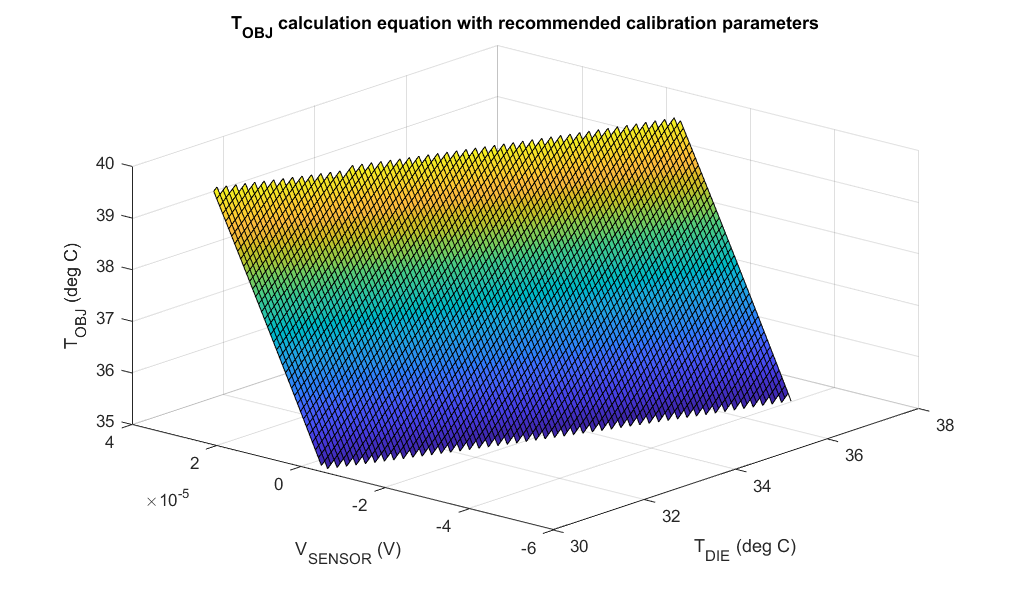
\includegraphics[scale=0.65]{figs/RecommendedTempCurve.png}
   \caption{Plot the the T\textsubscript{OBJ} equation with recommended calibration parameters and over the operating temperature range of the Ear-Monitor}
   \label{fig:RecommendedTempCurve}
\end{figure}


This linear characteristic of the TMP006 in the operating temperature range of the Ear-Monitor can be used to simplify the T\textsubscript{OBJ} calculation method as described in Equations \ref{eq:TempCurve1} to \ref{eq:TempCurve4}. These bulky recommended equations can be replaced by a first degree polynomial formula for a flat plane as described by:

\begin{equation}
\label{eq:FlatPlane}
T_{OBJ}=P0+P1\cdot T_{DIE}+P2\cdot V_{SENSOR}
\end{equation}

Where $P0$, $P1$ and $P2$ are parameters to be determined by a calibration process that follows the trial stage.

\subsection{PPG signal processing}


